\documentclass[12pt, a4paper, titlepage]{article}
\usepackage{amsthm}
\usepackage{amsmath}
\usepackage{amsfonts}
\usepackage{amssymb}
\setlength{\textwidth}{6.25in}
\usepackage{graphicx}
\usepackage{xcolor}
\usepackage{listings}
\lstset{numbers=none,
numberstyle=\tiny,
keywordstyle=\color{blue!70}, 
commentstyle=\color{red!50!green!50!blue!50},
frame=shadowbox,
rulesepcolor=\color{red!20!green!20!blue!20},
basicstyle=\ttfamily\small,
escapeinside=`', %将中文放在`和'之间,可以在lstlisting环境中准确的显示中文
}
\title{Financial Data Analysis Group Project\\
}
\author{Yufei Li  \\
	32014150004  \\
	\and 
	Yinan Wu \\
	32014150003 \\
	\and
	Ke Zhang\\
	32014150002\\
	\and
	Tianyunzi Chen\\
	32014020199
	}

\date{} 

\begin{document}
\maketitle

\begin{abstract}

\end{abstract}

\tableofcontents 
\newpage

\section{Introduction}
Exchange rate 
The Central Committee and the State Council promulgated the reform of the CNY exchange rate formation mechanism on July 21, 2005. The CNY exchange rate was no longer pegged to a single dollar, and fluctuated according to the market supply and demand. After August 11, 2015, the correlation between the CNY and the dollar index has declined. In 2016, the annual depreciation of CNY is about 6.67\%, against a basket of currency depreciation rate is 5.13\%. But the degree of marketization of the CNY in 2016 significantly increased, and gradually drops out of the ``dollar anchor". CNY exchange rate change, as China's international financial relations and even the normal development of economic relations, is an important link and plays an increasingly important role. Therefore, it has a vital significance to correct analysis and forecast the exchange rate and its volatility for the economic subject of financial policy and investment and financing decision-making undoubtedly. Also, to predict the CNY exchange rate better, it is very important to choose a satisfactory model.\\

Many domestic scholars have studied this based on time series measurement method. Which model of ARIMA model, ARCH model or GARCH model is more appropriate for the exchange rate fluctuations has been controversial. The paper of Zhang Zhongjie (2005) suggested that the exchange rate change was fit into $ARIMA(2,4,5)$ model. Hui Xiaofeng (2005) argued that there was a GARCH effect in the time series of USD / CNY, and the $GARCH(1,1)$ model was suitable for USD / CNY modeling, Xu Shaoqiang and Li Yaming(2007) used the ARMA model to forecast the exchange rate of the euro and yen of a basket of currencies. Then calculated the future exchange rate of the yuan against the US dollar according to the CNY benchmark exchange rate formula, and the forecast results were carried out. Liu Shuling (2008) selected data of the changes in the daily parity of CNY against the US dollar from July 25, 2005 to November 1, 2007. It is estimated that the $GARCH(1,1)$ model and the $ARMA(1,1)$ model are all suitable. Zhai Aimei(2009) showed that the CNY exchange rate volatility had certain leverage effect and the CNY exchange rate did not have the characteristics of floating exchange rate regime through the TGARCH model empirical study. Luo Xun (2009) analysed the exchange rate volatility model established form the data after the reform of China's exchange rate system. The study shows that there existed ARCH effect in China's foreign exchange market and $GARCH(1,1)$ was suitable.\\

It is not difficult to find that the data of previous studies are mostly old, while the appropriation of the model will change with the background of the times and the change of the data. In recent years, the international situation has been changed largely, so we select the latest data ,daily data from July 2005 to June 2017 of CNY exchange rate, to empirically research on the ARCH model, ARIMA model and GARCH model and to compare which forecasting model of CNY is more suitable for China and the development situation of this time.\\

\section{Data Source and Data Description}
\subsection{Data Source}

\subsection{Data Description}
We first use monthly USD / CNY exchange rate data from 1981-01-01 to 2017-06-01 to plot a trend figure shown as figure \ref{monthly}. According with the news, China used to set fixed exchange rate mechanism before 2015-07-21, the volatility of exchange rate was small. After that date, China started exchange rate regime reforming: announced a move away from the US dollar peg and used a floating exchange rate. Thus in this paper we will mainly focus on analysing exchange rate after the reform.\\ 
\begin{figure}
\begin{center}
\caption{CNY/ USD Exchange Rate using monthly data}\label{monthly}
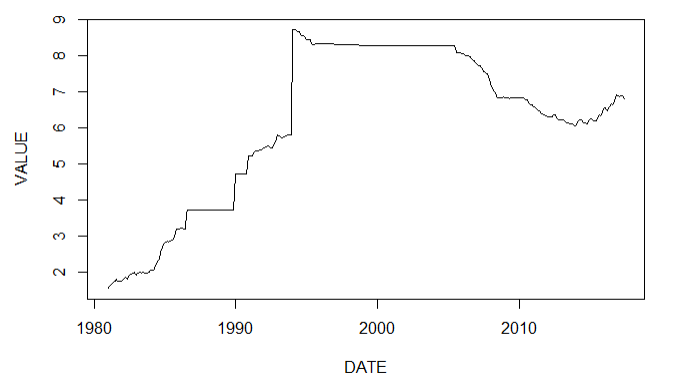
\includegraphics[width=0.6\textwidth]{monthly.png} 
\end{center}
\end{figure}

We collected the daily USD / CNY exchange rate as our data set. The data we found are already wipe out the seasonal effect so we use them directly in examining the model and further doing forecast. We divided the data into two parts one until July 21st,2016 for examine the model and the data after that date until June 9th,2017 for checking the evaluation of the models. The trend figure is shown in figure \ref{daily}.\\
\begin{figure}
\begin{center}
\caption{USD / CNY Exchange Rate using daily data}\label{daily}
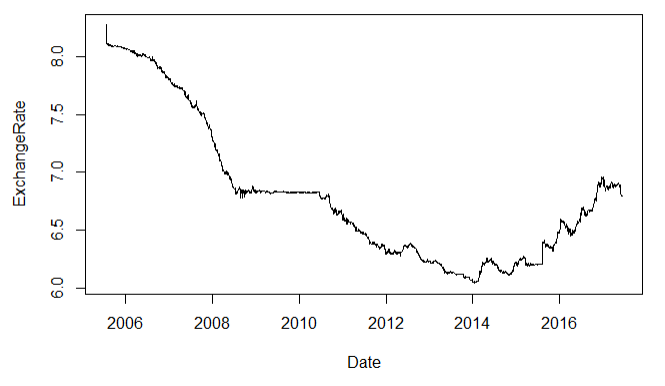
\includegraphics[width=0.6\textwidth]{daily.png} 
\end{center}
\end{figure}

\section{Model Specification}
There are usually two ways in analysing the exchange rate in time series: ARIMA model and GARCH model since they are the more general form of an ARMA model and an ARCH model. 

\subsection{Autoregressive Integrated Moving Average Model}
An Autoregressive Integrated Moving Average(ARIMA) model is a generalization of an Autoregressive Moving Average(ARMA) model with unit roots. Basically an ARMA model combines the ideas of Autocorrelation(AR) model and Moving Average(MA) model but it models with less number of parameters, achieving parsimony in the model. The general $ARMA(p,q)$ form is like $r_t = \phi_0 + \sum_{i=1}^p \phi_i r_{t-i} + a_t - \sum_{i=1}^q \theta_i a_{t-i}$ where ${a_t}$ is a white noise series. An AR model forms a multiple linear regression model with lagged values serving as the explanatory variables. A MA model is an infinite-order AR model with some parameter constraints. And the ``I" of Integrated indicates data values have been replaced with the difference between their values and the previous values.\\

To begin with, we want to check if the daily exchange rate series exists an unit root in the serial. As mentioned before, we first use the first $2766$ data (from 2005-07-21 to 2016-07-21) to check the ACF of series. From figure \ref{ACF}, we can say that ACF shows a strong autocorrelation which almost does not decay indicates the existence of unit root. We also run an ADF-test double-check the unit-root result. The ADF-test statistic is $-3.1048$ with p-value $0.0274$, which is larger than 0.01, so the unit-root hypothesis cannot be rejected under 1\% significant level.\\
\begin{figure}[h!]
\begin{center}
\caption{ACF results of exchange rate series}\label{ACF}
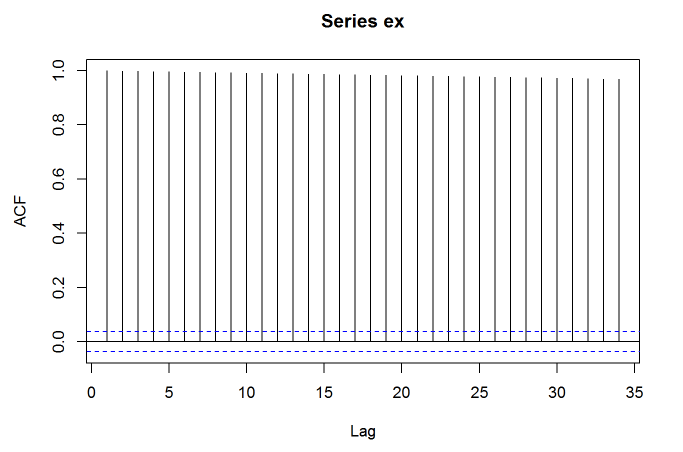
\includegraphics[width=0.6\textwidth]{ex_acf.png} 
\end{center}
\end{figure}
\begin{lstlisting}[language=R] 
origin=da$ExchangeRate
ex=origin[1:2766] # 2005-07-21 To 2016-07-21
acf(ex)
pacf(ex)

# ADF Test
adfTest(ex,lags=m1$order,type=c("c"))
## 
## Title:
##  Augmented Dickey-Fuller Test
## 
## Test Results:
##   PARAMETER:
##     Lag Order: 12
##   STATISTIC:
##     Dickey-Fuller: -3.1048
##   P VALUE:
##     0.0274 
\end{lstlisting}

However, when we want to further estimate a ARIMA model, the autocorrelation between the 8th difference exchange rate are still significant at lag 13th. Unlike Zhang(2005) who successfully estimated am $ARIMA(2,4,5)$ model using monthly data from Jan. 1989 to Dec.2003, we try to estimate an $ARIMA(6,4,12)$ model with unideal results. Thus, we focus on ARCH and GARCH model in the following research.

\subsection{General Autoregressive Conditional Heteroscedastic Model}
A General Autoregressive Conditional Heteroscedastic(GARCH) model is an extension of Autoregressive Conditional Heteroscedastic(ARCH) model. It shows the parsimonious of the parameters to adequately describe the volatility process of a series. The most commonly used GARCH model is $GARCH(1,1)$, and its form is like $a_t = \sigma_t \epsilon_t$, $\sigma^2 = \alpha_0 + \alpha_1 a_{t-1}^2 + \beta_1 \sigma_{t-1}^2$ where $0 \leq \alpha_1, \beta_1 \leq 1, (\alpha_1 + \beta_1) <1$. 

\section{Estimation and Result Analysis}

\section{Conclusions}\label{conclusions}
There is no longer \LaTeX{} example which was written by \cite{doe}.

\section{Reference}
\begin{thebibliography}{9}
\bibitem[Doe]{doe} \emph{First and last \LaTeX{} example.},
John Doe 50 B.C.
 
\end{thebibliography}

\section{Appendix}
\subsection{Additional R code}
\begin{lstlisting}[language=R] 
library(readxl)
library(timeDate)
library(timeSeries)
library(TSA)
library(fUnitRoots)
library(forecast)

data <- read_excel("D:/Junior/GitHub/FDA_project_LYF/Data/MonthlyData.xls")

head(data)
dim(data)

plot(data,type="l")

da <- read_excel("D:/Junior/GitHub/FDA_project_LYF/Data/DailyData.xlsx")

head(da)
dim(da)

plot(da,type="l")

# Take difference
dex2=diff(dex)
dex3=diff(dex2)
dex4=diff(dex3)
dex5=diff(dex4)
dex6=diff(dex5)
dex7=diff(dex6)
dex8=diff(dex7)
acf(dex8)
pacf(dex8)

#ARIMA
m2=arima(ex,c(6,4,12))
m2
Box.test(m2$residuals,lag=30,type = "Ljung")
pv2=1-pchisq(776.93,12)
pv2


Call:
arima(x = ex, order = c(6, 4, 12))

Coefficients:
          ar1      ar2     ar3      ar4     ar5      ar6      ma1     ma2
      -0.8638  -0.1001  0.0419  -0.0185  0.0187  -0.0084  -1.6103  0.3084
s.e.      NaN      NaN     NaN      NaN     NaN   0.0004      NaN  0.0003
         ma3      ma4     ma5     ma6     ma7      ma8     ma9    ma10     ma11
      0.2579  -0.0777  0.1486  -0.033  0.0986  -0.0976  0.1079  -0.095  -0.1169
s.e.     NaN      NaN  0.0001     NaN  0.0002      NaN     NaN     NaN   0.0004
        ma12
      0.1103
s.e.  0.0003

sigma^2 estimated as 0.0001398:  log likelihood = 8328.14,  aic = -16620.28

	Box-Ljung test

data:  m2$residuals
X-squared = 776.93, df = 30, p-value < 2.2e-16
\end{lstlisting}
\end{document}
